% Figure~\ref{fig:measurement_uncertainty_decomposition}
% (Section 4, Phase 2: components of measurement uncertainty of ML-based
% measurement systems).
%
% Replaces measurement_uncertainty_decomposition.png. Two macro-components
% (physical-quantity and measurement-model uncertainty), each with its
% contributions; symbols as in Eqs. (combined_std_uncertainty) and
% (model_uncertainty_decomposition):
%   u_c^2 = u_physical^2 + u_model^2,
%   u_model^2 = u_training^2 + u_architecture^2 + u_calibration^2.
% Finite and non-representative training data has no term of its own: it
% acts through training-process variability and through the approximation
% and generalization effects assessed by calibration on reference values.
%
% Compiles with plain pdflatex to a tightly-cropped vector PDF.
% Okabe-Ito colours: bluish green = physical-quantity branch (as the
% covariance propagation in Figure 1), reddish purple = measurement-model
% branch.
\documentclass{article}
\usepackage{amsmath}
\usepackage{amssymb}
\usepackage{tikz}
\usetikzlibrary{arrows.meta, positioning, calc}

\definecolor{okGreen}{HTML}{009E73}
\definecolor{okPurple}{HTML}{CC79A7}

\pagestyle{empty}
\hyphenpenalty=10000
\exhyphenpenalty=10000
\newsavebox{\figbox}
\newlength{\figborder}
\setlength{\figborder}{4pt}

\newcommand{\uphys}{u_{\mathrm{physical}}}
\newcommand{\umodel}{u_{\mathrm{model}}}

\begin{document}
\begin{lrbox}{\figbox}%
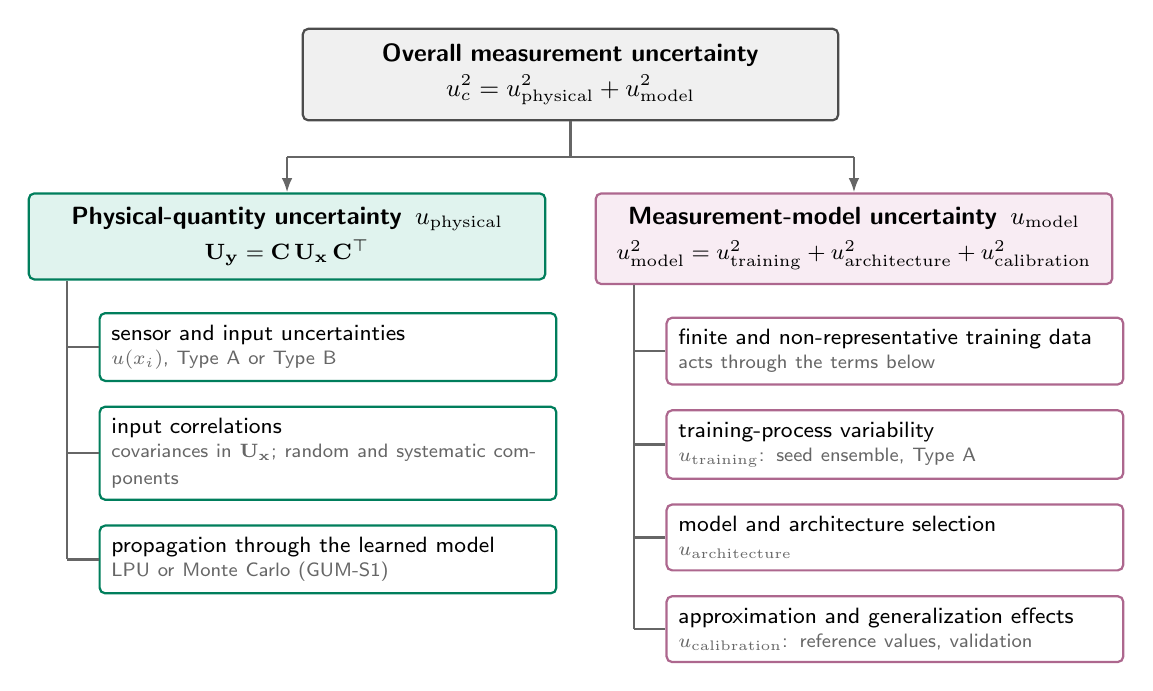
\begin{tikzpicture}[
  font=\sffamily\footnotesize,
  root/.style={rectangle, rounded corners=2pt, draw=black!70, thick, fill=black!6,
    text width=64mm, align=center, inner sep=2mm, font=\sffamily\small},
  macroP/.style={rectangle, rounded corners=2pt, draw=okGreen!80!black, thick, fill=okGreen!12,
    text width=62mm, align=center, inner sep=1.8mm, font=\sffamily\small},
  macroM/.style={rectangle, rounded corners=2pt, draw=okPurple!85!black, thick, fill=okPurple!14,
    text width=62mm, align=center, inner sep=1.8mm, font=\sffamily\small},
  leafP/.style={rectangle, rounded corners=2pt, draw=okGreen!80!black, fill=white, thick,
    text width=55mm, align=left, inner sep=1.5mm, minimum height=8mm},
  leafM/.style={rectangle, rounded corners=2pt, draw=okPurple!85!black, fill=white, thick,
    text width=55mm, align=left, inner sep=1.5mm, minimum height=8mm},
  sym/.style={font=\scriptsize, text=black!60},
  line/.style={thick, draw=black!60},
]
% ---------------- root ----------------
\node[root] (root) at (0,0)
  {\textbf{Overall measurement uncertainty}\\[0.5mm]
   \mbox{$u_c^2 = \uphys^2 + \umodel^2$}};

% ---------------- macro-components ----------------
\node[macroP, anchor=north] (P) at ($(root.south)+(-36mm,-9mm)$)
  {\textbf{Physical-quantity uncertainty}\enspace $\uphys$\\[0.5mm]
   {\footnotesize\mbox{$\mathbf{U}_{\mathbf{y}} = \mathbf{C}\,\mathbf{U}_{\mathbf{x}}\,\mathbf{C}^{\top}$}}};
\node[macroM, anchor=north] (M) at ($(root.south)+(36mm,-9mm)$)
  {\textbf{Measurement-model uncertainty}\enspace $\umodel$\\[0.5mm]
   {\footnotesize\mbox{$\umodel^2 = u_{\mathrm{training}}^2 + u_{\mathrm{architecture}}^2 + u_{\mathrm{calibration}}^2$}}};
\draw[line] (root.south) -- ++(0,-4.5mm) coordinate (rj);
\draw[line] (rj -| P.north) -- (rj -| M.north);
\draw[line, -{Latex[length=1.8mm]}] (rj -| P.north) -- (P.north);
\draw[line, -{Latex[length=1.8mm]}] (rj -| M.north) -- (M.north);

% ---------------- physical-quantity contributions ----------------
% leaves hang from a vertical spine on the left of each branch
\coordinate (Ps) at ($(P.south west)+(5mm,0)$);
\foreach \i/\txt/\note in {%
  1/{sensor and input uncertainties}/{$u(x_i)$, Type A or Type B},%
  2/{input correlations}/{covariances in $\mathbf{U}_{\mathbf{x}}$; random and systematic components},%
  3/{propagation through the learned model}/{LPU or Monte Carlo (GUM-S1)}} {
  \ifnum\i=1 \coordinate (Pprev) at ($(Ps)+(4mm,-1mm)$); \else \coordinate (Pprev) at ($(P\the\numexpr\i-1\relax.south west)$); \fi
  \node[leafP, anchor=north west] (P\i) at ($(Pprev)+(0,-3mm)$)
    {\txt\\[-0.3mm]{\scriptsize\color{black!60}\note}};
  \draw[line] (Ps |- P\i.west) -- (P\i.west);
}
\draw[line] (Ps) -- (Ps |- P3.west);

% ---------------- measurement-model contributions ----------------
\coordinate (Ms) at ($(M.south west)+(5mm,0)$);
\foreach \i/\txt/\note in {%
  1/{finite and non-representative training data}/{acts through the terms below},%
  2/{training-process variability}/{$u_{\mathrm{training}}$: seed ensemble, Type A},%
  3/{model and architecture selection}/{$u_{\mathrm{architecture}}$},%
  4/{approximation and generalization effects}/{$u_{\mathrm{calibration}}$: reference values, validation}} {
  \ifnum\i=1 \coordinate (Mprev) at ($(Ms)+(4mm,-1mm)$); \else \coordinate (Mprev) at ($(M\the\numexpr\i-1\relax.south west)$); \fi
  \node[leafM, anchor=north west] (M\i) at ($(Mprev)+(0,-3mm)$)
    {\txt\\[-0.3mm]{\scriptsize\color{black!60}\note}};
  \draw[line] (Ms |- M\i.west) -- (M\i.west);
}
\draw[line] (Ms) -- (Ms |- M4.west);

\end{tikzpicture}%
\end{lrbox}%
% crop the page to the picture
\pdfpagewidth=\dimexpr\wd\figbox+2\figborder\relax
\pdfpageheight=\dimexpr\ht\figbox+\dp\figbox+2\figborder\relax
\pdfhorigin=\figborder
\pdfvorigin=\figborder
\shipout\hbox{\usebox{\figbox}}
\end{document}
